\documentclass{article}
\usepackage[british]{babel}
\usepackage{graphicx}
\documentclass[a4paper, 11pt]{article}
\usepackage[top=3cm, bottom=3cm, left = 2cm, right = 2cm]{geometry} 
\geometry{a4paper} 
\usepackage[utf8]{inputenc}
\usepackage[skip=2pt]{caption}

\begin{document}

\title{Report}

\author{Musawer Hussain, Vladimir Volgin, Oleg Tretieu}

\maketitle

\

\begin{figure}[h]
  \centering
  \caption{Decision tree}
  \raisebox{0.0\height}{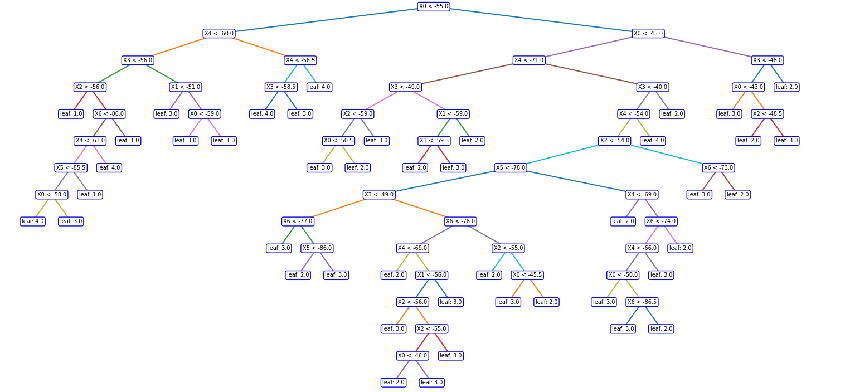
\includegraphics[width=14.2540994359176cm,height=6.58685884822248cm]{report-1.pdf}}
\end{figure}
\\

\section{Clean data set}
  \\

\renewcommand{\arraystretch}{2}
\begin{table}[htb]
  \centering
  \caption{Confusion matrix for clean dataset} \\
  \begin{tabular}{|l|l|l|l|l|}
  \hline
                & Room 1 predicted & Room 2 predicted & Room 3 predicted & Room 4 predicted \\ \hline
  Room 1 actual & 495              & 0                & 2                & 3                \\ \hline
  Room 2 actual & 0                & 478              & 22               & 0                \\ \hline
  Room 3 actual & 2                & 18               & 478              & 2                \\ \hline
  Room 4 actual & 5                & 0                & 1                & 494              \\ \hline
  \end{tabular}
\end{table}
\\

\textbf{Accuracy:} 0.9685 \\
\\
\textbf{Recall:} \\
Room 1: 0.98867706 \\
Room 2: 0.95791808 \\
Room 3: 0.94327441 \\
Room 4: 0.98443314 \\
\\
\\
\textbf{Precision:} \\
Room 1: 0.98034611 \\
Room 2: 0.95797757 \\
Room 3: 0.9460876 \\
Room 4: 0.98566303 \\
\\
\textbf{F1-measures:} \\
Room 1: 0.98406375 \\
Room 2: 0.958  \\
Room 3: 0.9448345 \\
Room 4: 0.98698699 \\
\\

\section{Noisy data set}
  \\

\renewcommand{\arraystretch}{2}  
\begin{table}[htb]
  \centering
  \caption{Confusion matrix for noisy dataset} \\
  \begin{tabular}{|l|l|l|l|l|}
  \hline
                & Room 1 predicted & Room 2 predicted & Room 3 predicted & Room 4 predicted \\ \hline
  Room 1 actual & 379              & 49               & 19               & 43               \\ \hline
  Room 2 actual & 29               & 398              & 47               & 23               \\ \hline
  Room 3 actual & 30               & 37               & 410              & 38               \\ \hline
  Room 4 actual & 47               & 30               & 37               & 384              \\ \hline
  \end{tabular}
\end{table}
\\

\textbf{Accuracy:} 0.7855000000000001 \\
\\
\textbf{Recall:} \\
Room 1: 0.77275535 \\
Room 2: 0.80197697 \\
Room 3: 0.79740095 \\
Room 4: 0.77106065 \\
\\
\textbf{Precision:} \\
Room 1: 0.78238612 \\
Room 2: 0.77477728 \\
Room 3: 0.79695117 \\
Room 4: 0.78396774 \\
\\
\textbf{F1-measures:} \\
Room 1: 0.7774359 \\
Room 2: 0.78733927  \\
Room 3: 0.79766537 \\
Room 4: 0.77890467 \\

\pagebreak

\section{Analysis}

When using the clean data, the vast majority of the rooms are identified
correctly. We see from the confusion matrix that the rooms which were most
often confused with eachother are Room 2 and Room 3. With the noisy data,
while most rooms are still correctly recognised, there is a significant
amount of incorrect classifications. Most notably: Room 1 often gets misclassified as
Room 2, Room 4 as Room 1, and Room 2 as Room 3.
\

The performance on the noisy dataset is significantly worse than on the clean
dataset, which we can see by comparing the evaluation metrics above. This
could be caused by the decision tree overfitting when training on the noisy
data, effectively ``learning the noise'', which leads to worse generalisation.
Furthermore, the noisy dataset is slightly unbalanced, as Room 3 has 515
samples, whereas Room 1 only has 490, so it is necessary to look at the
normalized confusion matrix.


\end{document}
